%! suppress = LineBreak
\section{Оружие, основанное на системе частиц}\label{sec:WeaponIdea}

Оружие, генерируемое системой, основано на идее из программы NEAT Particles\cite{s2,s3}. Каждое оружие содержит в себе нейронную сеть (Рисунок~\ref{Weapon}). Каждый кадр анимации каждая частица, выпущенная из оружия, подает на вход в нейронную сеть:

\begin{enumerate}
    \item {\small \textbf{RelativePos.x}} -- координата $x$ текущего положения частицы относительно точки выстрела.
    \item {\small \textbf{RelativePos.y}} -- координата $y$ текущего положения частицы относительно точки выстрела.
    \item {\small \textbf{DistanceFromOrigin}} -- расстояние от точки выстрела.
\end{enumerate}

После этого нейронная сеть активируется и выводит для этого анимационного кадра:

\begin{enumerate}
    \item {\small \textbf{x}} -- координата $x$ вектора скорости или силы, приложенной к частице.
    \item {\small \textbf{y}} -- координата $y$ вектора скорости или силы, приложенной к частице.
    \item {\small \textbf{hue}} -- компонента цвета частицы в модели HSV\@.
    \item {\small \textbf{maxSpeed}} -- максимальная скорость частицы.
    \item {\small \textbf{force}} -- длина вектора скорости частицы или силы, действующей на неё.
\end{enumerate}


\begin{figure}[ht]
    \begin{center}
        \scalebox{0.17}{
            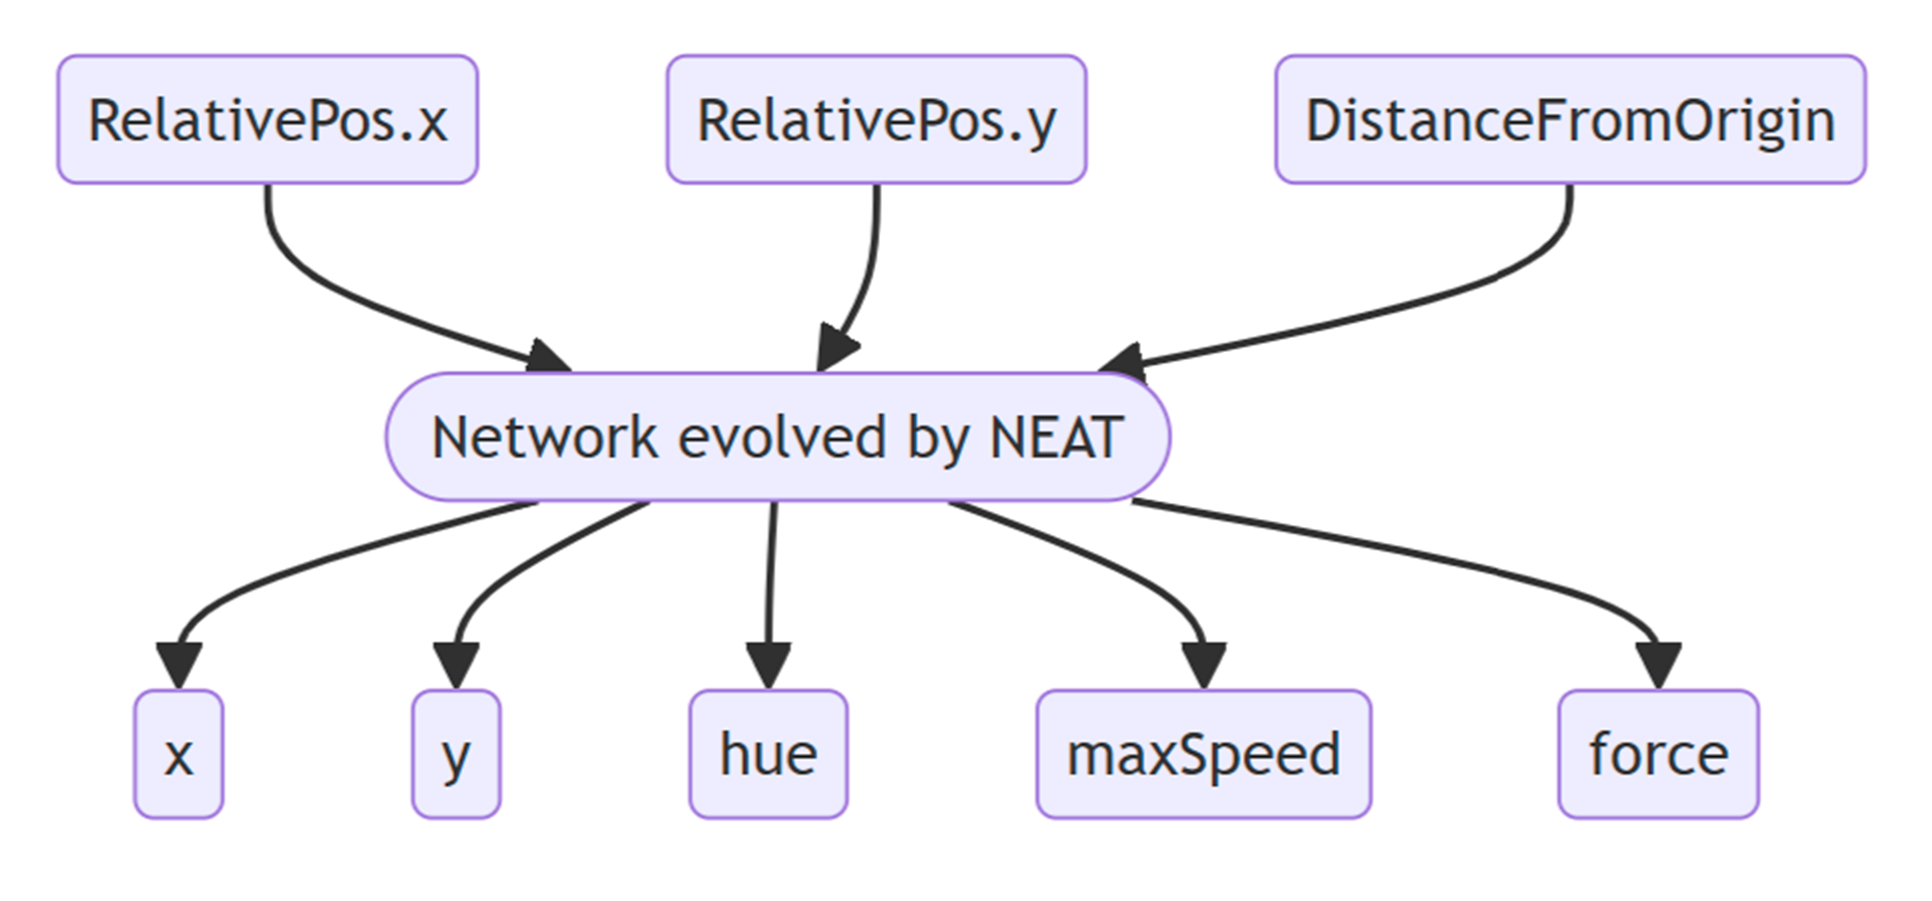
\includegraphics{images/GenIdea}
        }

        \caption{
            \label{Weapon}
            Как нейронная сеть управляет снарядами.}
    \end {center}
\end {figure}


Поскольку оружие представляется нейронной сетью, можно генерировать новое оружие, изменяя веса или топологию нейронной сети. Выбор алгоритма для этого обосновывается в следующей главе.
